\documentclass{article}
\usepackage{tikz}

\usepackage{pgfplots}
\usepackage{xcolor}
\begin{document}
   \begin{figure}
    \centering

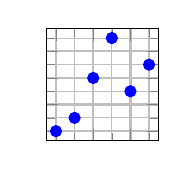
\begin{tikzpicture}
  \begin{axis}[
    % xlabel=$x$,
    % ylabel=$c_x$,
xticklabels=\empty,
    yticklabels=\empty,
    grid=both,
    minor tick num=1, % Number of minor ticks per major tick
    major grid style={line width=0.8pt,draw=gray!50},
    width=3cm,
    height=3cm,
    legend style={at={(1,1)},anchor=north east}
  ]
    % Scatter plot points
    \addplot[
      only marks,
      mark=*,
      color=blue,
      mark size=2pt
    ] coordinates {
      (0,0) (1,0.1) (2,0.4) (3,0.7) (4,0.3) (5,0.5)
    };
    % \addlegendentry{Data points}
    
    % Polynomial approximation (e.g., quadratic)
    % \addlegendentry{Polynomial approximation}
  \end{axis}
\end{tikzpicture}
\begin{tikzpicture}[overlay]
\node at (0.75,1.2) {\small \textbf{Piecewise}};
\draw[->, thick] (0.25,0.9) -- (1.25,0.9); % Adjust coordinates as needed
\node at (0.8,0.6) {approx.};
\node at (-0.85,2) {\textit{Target State}};
  \node at (2.4,2.25) {\textit{\shortstack{Polynomial \\approximation}}};
\end{tikzpicture}
\hspace{1.25cm}
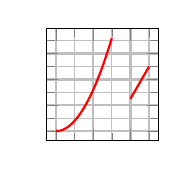
\begin{tikzpicture}
  \begin{axis}[
    % xlabel=$x$,
    % ylabel=$p(x)$,
    xticklabels=\empty,
    yticklabels=\empty,
    grid=both,
    minor tick num=1, % Number of minor ticks per major tick
    major grid style={line width=0.8pt,draw=gray!50},
    width=3cm,
    height=3cm,
    legend style={at={(1,1)},anchor=north east}
  ]

    % Polynomial approximation (e.g., quadratic)
    \addplot[
      domain=0:3,
      samples=100,
      color=red,
      thick
    ] {0.08*x^2};
    \addplot[
      domain=4:5,
      samples=100,
      color=red,
      thick
    ] {0.25*(x-3)};
    % \addlegendentry{Polynomial approximation}
  \end{axis}
\end{tikzpicture}
\hspace{0.25cm}
\begin{tikzpicture}[overlay]
\node at (0.5,1.2) {\small \textbf{Piecewise}};
\draw[->, thick] (0,0.9) -- (1,0.9); % Adjust coordinates as needed
\node at (0.5,0.6) {QSVT};
  \node at (2.2,2) {\textit{Prepared State}};
\end{tikzpicture}
\hspace{1cm}
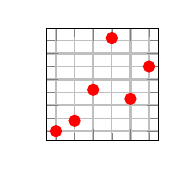
\begin{tikzpicture}
  \begin{axis}[
    % xlabel=$x$,
    % ylabel=$c'_x$,
    xticklabels=\empty,
    yticklabels=\empty,
    grid=both,
    minor tick num=1, % Number of minor ticks per major tick
    major grid style={line width=0.8pt,draw=gray!50},
    width=3cm,
    height=3cm,
    legend style={at={(1,1)},anchor=north east}
  ]
    % Scatter plot points
    \addplot[
      only marks,
      mark=*,
      color=red,
      mark size=2pt
    ] coordinates {
      (0,0) (1,0.08) (2,0.32) (3,0.72) (4,0.25) (5,0.5)
    };
  \end{axis}
\end{tikzpicture}
\end{figure}
\end{document}